\chapter{Beyond the threshold}
\label{ch:giant}

Chapter~\ref{ch:percolation} located the threshold but said nothing about the
size of the giant component. The tensor $A$ is built from four matrices of first
moments; the map needs whole generating functions. The threshold therefore uses
strictly less information than the map, and in this chapter we ask what the
rest of that information buys. The results are reported here for the first
time; where they extend the percolation map of
\citet{vazquez2023pre,vazquez2024comnet} the debt is marked at the point of use.

What it buys is a hierarchy, Table~\ref{tab:hierarchy}, and an unusually clean
one: each additional order of moment data buys exactly one more thing about the
transition.

\begin{table}[b]
\centering\small
\begin{tabular}{ll}
\hline\hline
quantity & input required\\
\hline
threshold $\theta$, $\Lambda$ & first moments\\
critical amplitude $B$ & $+$ second moments\\
$S$ away from the threshold & the generating functions\\
\hline\hline
\end{tabular}
\caption{\textbf{What each level of input determines.} The threshold needs the
four moment matrices of Sec.~\ref{sec:ensembles} and nothing else. One further
order of moments fixes the slope with which the giant component grows out of
the threshold. Nothing short of the full distributions fixes its size away from
there.}
\label{tab:hierarchy}
\end{table}

Establishing the hierarchy needs one structural observation, made in
Sec.~\ref{sec:jacobian}, and everything else follows from it. This chapter also
lifts an assumption that has been in force since Sec.~\ref{sec:ensembles} ---
that a complex's participation in one layer says nothing about its
participation in another --- and shows that lifting it matters more than one
might expect.

\section{The threshold is a Jacobian}
\label{sec:jacobian}
\index{threshold tensor}
\index{Jacobian}

Differentiate the map, Eqs.~\eqref{eq:Qminus}--\eqref{eq:Qplus}, at the trivial
fixed point $Q\equiv1$. Every generating function equals one there, so each
product leaves a single first derivative, and by Eq.~\eqref{eq:moments} each of
those is an entry of one of the four moment matrices. Comparing the result with
the tensor of Sec.~\ref{sec:threshold} entry by entry gives
\begin{equation}
  \mathrm{vec}^{2}A=I-J,
  \qquad
  J_{ab}=\frac{\partial F_{a}}{\partial Q_{b}}\bigg|_{Q=1},
  \label{eq:AisJ}
\end{equation}
where $F$ is the map. The published threshold tensor \emph{is} the Jacobian of
the map at its trivial fixed point. Consequently
\begin{equation}
  \Lambda=\lambda-1,
  \label{eq:Lambdalambda}
\end{equation}
with $\lambda$ the Perron root of $J$: the threshold calculation is the
statement that $Q\equiv1$ loses stability, exactly as
Sec.~\ref{sec:percolation-intro} said it should be.

The four blocks of $A$ acquire a plain reading from this. They are the four ways
of composing a step with the state it lands in --- up then up, up then down,
down then up, down then down --- and the Kronecker deltas $\delta_{mk}$ that
select the excess averages are precisely the brackets $[\,\cdot\,]_{k=m}$ of
Fig.~\ref{fig:themap}, which is to say the rule that the arriving inclusion is
discounted only from routes back into the layer it came from. Nothing in $A$ was
ever arbitrary.

The observation is small and it carries the chapter: threshold and order
parameter are not two calculations but two orders of one, on the same index set and in the same layout. Everything in this chapter is
obtained by carrying that expansion further or by changing what is expanded.

\section{What the first moments do not determine}
\label{sec:degeneracy}
\index{null model}

Since $A$ depends on the ensemble only through first moments, and moments do not
determine a distribution, $S$ cannot be a function of $A$. The size of the
degeneracy is measured below.

Take two graphs whose degree distributions are
\begin{align}
  P_{A}(k)&=0.5\,\delta_{k,0}+0.5\,\delta_{k,4},\nonumber\\
  P_{B}(k)&=0.2\,\delta_{k,0}+0.5\,\delta_{k,1}+0.3\,\delta_{k,5}.
  \label{eq:PAPB}
\end{align}
Both have $\ave{k}=2$ and $\ave{\bar k}=3$. They therefore have identical
$\theta=3p-1$, identical $\Lambda$, and the identical site percolation threshold
$p_{c}=1/3$ --- every entry of the threshold tensor agrees. At $p=1$ the first
has $S=0.500$ and the second $S=0.673$ (Fig.~\ref{fig:degeneracy}). Nothing in
Chapter~\ref{ch:percolation} can tell them apart, and they differ by a third.

\begin{figure}[t]
\centering
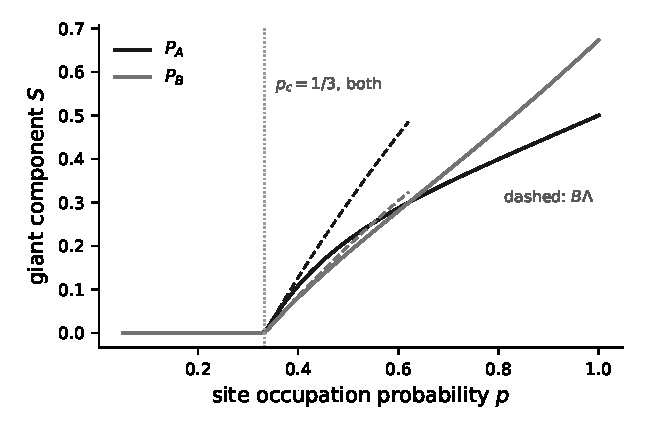
\includegraphics[width=0.9\linewidth]{figs/fig-degeneracy.pdf}
\caption{\textbf{First moments do not determine the order parameter.} Site
percolation on two configuration-model graphs with the degree distributions of
Eq.~\eqref{eq:PAPB}, which share $\ave{k}=2$ and $\ave{\bar k}=3$ and hence
share every entry of the threshold tensor. They share the threshold $p_{c}=1/3$
and nothing else: the order parameter differs everywhere above it, and so does
the slope with which it leaves. Dashed lines are the leading behaviour
$B\Lambda$ of Eq.~\eqref{eq:Bgraph}, $B=4/3$ and $B=8/9$. Generated by
\code{figs/\allowbreak beyond\_\allowbreak threshold.\allowbreak py}.}
\label{fig:degeneracy}
\end{figure}

The extra input is nonetheless cheap, and this is the practical point. Every
example in Chapter~\ref{ch:percolation} was built from a distribution and then
projected onto its mean. The bond-percolated triangle is the clearest case: the
enumeration in Sec.~\ref{sec:structurebystructure} produced a whole
distribution over excess component sizes, of which $\bar
s_{\triangle}(q)=2q(1+q-q^{2})$ was only the mean. Written as a generating
function it is
\begin{equation}
  \begin{aligned}
    \bar G_{\triangle}(y)&=\bigl(3q^{2}-2q^{3}\bigr)y^{2}+2q(1-q)^{2}y\\
    &\quad+(1-q)^{3}+q(1-q)^{2}.
  \end{aligned}
  \label{eq:tripgf}
\end{equation}
Un-projecting is a one-line change per model. And for Poisson distributions
there is nothing to un-project, since $\Phi=\bar\Phi=e^{\ave{\kappa}(x-1)}$ is
already fixed by its mean.

\citet{vazquez2024comnet} gives the mean intra-complex component size
of a triangle --- as opposed to the \emph{excess} size, which is what the
threshold uses --- with $3/2$ on the single-link term. It should be $5/3$: in the configuration
with one bond present the three members sit in components of sizes $2$, $2$
and $1$, so a member chosen at random is in a component of mean size
$(2+2+1)/3=5/3$, not $3/2$. Weighting each configuration by its probability,
\begin{align*}
  s_{\triangle}(q)&=3\bigl[q^{3}+3q^{2}(1-q)\bigr]
    +\tfrac{5}{3}\bigl[3q(1-q)^{2}\bigr]+1\cdot(1-q)^{3}\\
  &=3\bigl(q^{3}+3q^{2}(1-q)\bigr)+5q(1-q)^{2}+(1-q)^{3},
\end{align*}
the $5/3$ and the $3$ multiplying out to the $5$ in the collapsed form. That
is $s_{\triangle}=1+\bar s_{\triangle}=1+2q(1+q-q^{2})$, which is what
Eq.~\eqref{eq:tripgf} returns.

The published threshold is unaffected, for a definite reason:
$\ave{s}_{20}$ never enters $\theta$ at all, because triangles are never reached
from above --- nothing includes a triangle. The coefficient does enter the order
parameter of the triangle layer, $S_{2}$. Both forms are in \code{figs/\allowbreak triangles\_\allowbreak vs\_\allowbreak regular.\allowbreak py}, which enumerates the triangle rather than quoting it.

\section{The critical amplitude}
\label{sec:amplitude}
\index{critical amplitude|textbf}
\index{order parameter}

Between ``first moments'' and ``the whole distribution'' there is one more rung,
and it is reached by carrying the expansion of Sec.~\ref{sec:jacobian} to second
order.

Write $Q=1-x$ and expand the map about the trivial fixed point,
\[
  x_{a}=\sum_{b}J_{ab}x_{b}-\tfrac12\sum_{bc}M_{abc}x_{b}x_{c}+O(x^{3}),
\]
with $M_{abc}=\partial^{2}F_{a}/\partial Q_{b}\partial Q_{c}$ at $Q=1$. Let $r$
and $\ell$ be the right and left Perron vectors of $J$, normalised so that
$\ell\cdot r=1$. Just above threshold $\lambda=1+\Lambda$ with
$\Lambda\to0^{+}$; putting $x=\epsilon r$ and projecting on $\ell$ annihilates
the linear term and leaves
\[
  \epsilon=\frac{2\Lambda}{C},\qquad C\equiv\ell\cdot M[r,r].
\]
Expanding Eq.~\eqref{eq:Sl} to first order then gives
\[
  S_{l}=B_{l}\Lambda+O(\Lambda^{2}),
  \qquad
  B_{l}=\frac{2\,\nabla P^{l}\cdot r}{C}.
\]
Only \emph{second} derivatives of the generating functions enter $B_{l}$: one
moment order beyond what $A$ needs, and no more. That is the middle row of
Table~\ref{tab:hierarchy}.

Two things make this practical rather than merely formal. The rank-three tensor
$M$ never has to be built, since contracting it twice with $r$ is a second
directional derivative, $M_{a}[r,r]=\frac{d^{2}}{dt^{2}}F_{a}(1+tr)|_{t=0}$ ---
an ordinary single-variable derivative of a product of generating functions. And
the $2L^{2}$ indices collapse: discarding iteratively every index whose row or
column of $J$ vanishes identically leaves a \emph{core} without changing the
non-zero spectrum. For a hypergraph that is $2$ indices of $8$; for a graph with
links and triangles, $4$ of $18$. In both cases the survivors are exactly the
unknowns one would have written down by hand. \code{amplitude.\allowbreak CriticalAmplitude} carries this: the directional derivative, the core reduction, and $B_{l}$.

Table~\ref{tab:amplitudes} collects the closed forms on the critical manifold.
The graph is worth doing by hand, because there the two indices collapse to the
single scalar of Sec.~\ref{sec:percolation-intro} and the whole of the recipe
above fits in four lines. Write $x=1-u$ for the probability that a link does
lead to the giant component. Then $u=1-pq+pq\,G_{1}(u)$ is
\[
  x=pq\Bigl[\ave{\bar k}\,x-\tfrac12\ave{\bar k(\bar k-1)}\,x^{2}\Bigr]
    +O(x^{3}),
\]
since $G_{1}(1-x)=1-\ave{\bar k}x+\tfrac12\ave{\bar k(\bar k-1)}x^{2}-\cdots$.
Dividing by $x$ and solving,
\[
  x=\frac{2\bigl(pq\ave{\bar k}-1\bigr)}{pq\ave{\bar k(\bar k-1)}}.
\]
The Perron root here is $\lambda=\sqrt{pq\ave{\bar k}}$ --- a square root
because a graph is two layers and the Jacobian carries the product across them
--- so $pq\ave{\bar k}=(1+\Lambda)^{2}$ and the bracket is $2\Lambda$ to leading
order. Finally $S=p\bigl[1-G_{0}(1-x)\bigr]\simeq p\ave{k}\,x$, and on the
critical manifold $pq\ave{\bar k}=1$, so
\begin{equation}
  \lambda=\sqrt{pq\ave{\bar k}},
  \qquad
  B=\frac{4p\,\ave{k}\ave{\bar k}}{\ave{\bar k(\bar k-1)}}.
  \label{eq:Bgraph}
\end{equation}
Only the second factorial moment of the excess degree entered, which is the
middle row of Table~\ref{tab:hierarchy} in the one case where it can be watched
happening. A Poisson degree distribution has
$\ave{\bar k(\bar k-1)}=\ave{k}^{2}$ and $\ave{\bar k}=\ave{k}$, giving $B=4p$,
the first row of Table~\ref{tab:amplitudes}.
The hypergraph goes the same way with one more generating function in the
chain, and for arbitrary degree and cardinality distributions it gives
\begin{equation}
  B=\frac{4p\,\ave{k}\ave{\bar k}\ave{\bar c}}
         {\ave{\bar c}\ave{\bar k(\bar k-1)}
          +p\ave{\bar k}^{2}\ave{\bar c(\bar c-1)}}.
  \label{eq:Bhyper}
\end{equation}
Equation~\eqref{eq:Bgraph} separates the two distributions of
Fig.~\ref{fig:degeneracy}: they agree on $\ave{k}$ and $\ave{\bar k}$ but have
$\ave{\bar k(\bar k-1)}=6$ and $9$, giving $B=4/3$ against $8/9$. Setting the
degree distribution Poisson gives $B=4p$, and at $p=q=1$ the
Erd\H{o}s--R\'enyi result $S\simeq2(\ave{k}-1)$.

\begin{table}[t]
\centering\small
\begin{adjustbox}{max width=\linewidth}
\begin{tabular}{lll}
\hline\hline
system & $\lambda$ & $B$\\
\hline
Poisson graph & $\sqrt{pq\ave{k}}$ & $4p$\\[2pt]
Poisson hypergraph & $\sqrt{pq\ave{k}\ave{c}}$ & $4p/(1+p\ave{c})$\\[2pt]
Poisson multiplex & $\bigl(\sum_{l}q_{l}\ave{k}_{l}\ave{c}_{l}\bigr)^{1/2}$
  & $4\big/\bigl(1+\sum_{l}q_{l}\ave{k}_{l}\ave{c}_{l}^{2}\bigr)$\\[2pt]
Poisson, triangles & $\bigl(q\ave{k}_{|}
  +2q(1{+}q{-}q^{2})\ave{k}_{\triangle}\bigr)^{1/2}$
  & $4\big/\bigl[1+2q^{2}(3-2q)\ave{k}_{\triangle}\bigr]$\\
\hline\hline
\end{tabular}
\end{adjustbox}
\caption{\textbf{Critical amplitudes} in $S=B\Lambda+O(\Lambda^{2})$, on the
critical manifold $\lambda=1$. Sites are present with probability $p$, bonds or
hyperedges with probability $q$. The arbitrary-distribution cases are
Eqs.~\eqref{eq:Bgraph} and~\eqref{eq:Bhyper}.}
\label{tab:amplitudes}
\end{table}

The last row of Table~\ref{tab:amplitudes} contains something the threshold
could not have shown. For bond percolation on a graph with links and triangles,
\begin{equation}
  B=\frac{4}{1+2q^{2}(3-2q)\ave{k}_{\triangle}},
  \label{eq:Btriangle}
\end{equation}
and $\ave{k}_{|}$ does not appear. The link layer moves the threshold but not
the amplitude. The reason is the fine-grained interior of
Sec.~\ref{sec:definition}: a link's excess component size is Bernoulli, its
generating function is affine, and an affine function has no second derivative
to contribute. At the level of $\theta$ the two layers enter symmetrically and
nothing suggests this. It is a distinction that only appears one order up.

\section{Where the expansion breaks down}
\label{sec:breakdown}
\index{interdependent networks|textbf}
\index{spinodal}

The denominator $C=\ell\cdot M[r,r]$ is a sum of non-negative terms, since
$\ell$, $r$ and all second derivatives of generating functions at $1$ are
non-negative. When it is finite and positive, the transition is continuous with
$S\propto\Lambda$ and order parameter exponent $\beta=1$. Both qualifications
carry weight.

\emph{$C$ can diverge.} Finiteness is a condition on second factorial moments of
the excess distributions --- again one order beyond $\theta$. For a graph
$C\propto\ave{\bar k(\bar k-1)}=\ave{k(k-1)(k-2)}/\ave{k}$, which diverges for a
scale-free degree distribution with exponent $\gamma\le4$. There
Eq.~\eqref{eq:Bgraph} returns $B\to0$: the linear branch has vanishing
amplitude, $\beta\ne1$, and one recovers the familiar $\beta=1/(\gamma-3)$ of
heterogeneous mean field for $3<\gamma<4$. The expansion announces its own
breakdown, but the closed forms of Table~\ref{tab:amplitudes} are statements about ensembles with finite second
moments and must not be quoted outside that range.

\emph{$C$ can vanish.} Then the map is affine along the critical direction and
there is no linear branch at all. The elementary case is the two-regular graph,
where $\bar\Phi(x)=x$ and there is no transition of this type. So $C$ is a
symbolic continuity criterion, computable alongside $\theta$ and $\Lambda$.

Its non-negativity settles something. It has recently been argued
\citep{keating2026} that group structure on its own produces only continuous
transitions. For anything in the percolation class this now has a one-line
proof: a complex contributes to $C$ through second derivatives of its
generating functions, and those cannot be negative. The qualifier \emph{on its
own} is doing work.
Section~\ref{sec:groupcontagion} maps a threshold rule to a chygraph and keeps
the recursion, but its intra-complex function is not a generating function in
the failure variable, and the onset can then be discontinuous.

One caveat delimits the scope, and it is an exclusion rather than a
technicality. Equations~\eqref{eq:Qminus}--\eqref{eq:Qplus} are the extinction
conditions of a multi-type branching process, and for such maps the loss of
stability of $Q\equiv1$ locates the transition. Interdependent networks
\citep{buldyrev2010,radicchi2015} are not of this class: their giant component
appears through a saddle-node bifurcation while $Q\equiv1$ is \emph{still
stable}, so $\Lambda=0$ does not locate the transition and the physical fixed
point has to be reached by a cascade from above rather than by iterating up from
$Q=0$. Mapping those constructions to chygraphs, and identifying what replaces
$\Lambda$ there, is not done.

\section{Dependent layers}
\label{sec:joint}
\index{correlated layers|textbf}

In this section we lift the factorisation assumption.
Section~\ref{sec:ensembles} took the generating functions to factorise over
target layers, $\Phi^{l}(x)=\prod_{k}\Phi^{l}_{k}(x_{k})$. That
covers every mapping in Chapter~\ref{ch:percolation}, and it is false for
anything in which a complex's participation in one layer is tied to its
participation in another: a node whose triangle count moves with its link count,
a hyperedge whose cardinalities in two vertex layers are correlated. Joint
degree distributions of exactly this kind are what the motif formalism of
\citet{mann2021} works with, and Chapter~\ref{ch:data} recommended
measuring the correlation rather than assuming it away.

Dropping the factorisation changes the \emph{status} of the excess generating
functions. They stop being independent inputs and become derivatives of the
joint one,
\begin{equation}
  \bar\Phi^{l,(m)}(x)=\frac{\partial\Phi^{l}/\partial x_{m}}
    {\left.\partial\Phi^{l}/\partial x_{m}\right|_{x=1}},
  \label{eq:excessderived}
\end{equation}
and likewise for $\bar G$. The map becomes
\begin{align}
  Q^{ml}_{-}&=\Phi^{l}\bigl(Q^{l\cdot}_{-}\bigr)\,
              \bar G^{l,(m)}\bigl(Q^{l\cdot}_{+}\bigr),\nonumber\\
  Q^{ml}_{+}&=\bar\Phi^{l,(m)}\bigl(Q^{l\cdot}_{-}\bigr)\,
              G^{l}\bigl(Q^{l\cdot}_{+}\bigr),
  \label{eq:jointmap}
\end{align}
reducing term by term to Eqs.~\eqref{eq:Qminus}--\eqref{eq:Qplus} when the
functions factorise.

Differentiating at $Q=1$, a second derivative of the joint function now stands
where the published tensor carried a first moment. Define the
\emph{inclusion-biased} moments
\begin{equation}
  \ave{\bar\kappa^{(m)}}_{lk}
   =\frac{\ave{\kappa_{lm}\bigl(\kappa_{lk}-\delta_{mk}\bigr)}}
         {\ave{\kappa_{lm}}},
  \label{eq:biased}
\end{equation}
and likewise $\ave{\bar s^{(m)}}$: the expected chy-degree to layer $k$ of a
complex \emph{reached through an inclusion into layer $m$}. That is the whole
generalisation. Unconditional first moments are replaced by inclusion-biased
second moments, and everything downstream --- the Jacobian, the determinant, the
fixed point --- is unchanged.

\subsection{Identical marginals, different transitions}

The correction is not small. The demonstration below holds the marginals fixed
exactly. Take bond percolation on a graph with links and triangles, and
three joint distributions of the number of links $k_{|}$ and triangles
$k_{\triangle}$ at a node, each with the marginals $k_{|}\in\{1,3\}$ and
$k_{\triangle}\in\{0,2\}$ with probability $1/2$:
\begin{align}
  \text{correlated:}&\quad(k_{|},k_{\triangle})\in\{(1,0),(3,2)\},\nonumber\\
  \text{anti-correlated:}&\quad(k_{|},k_{\triangle})\in\{(1,2),(3,0)\},\nonumber\\
  \text{independent:}&\quad\text{the product of the marginals.}
\end{align}
All three have $\ave{k}_{|}=2$, $\ave{\bar k}_{|}=3/2$,
$\ave{k}_{\triangle}=\ave{\bar k}_{\triangle}=1$, hence every entry of the
published threshold tensor agrees. Equation~\eqref{eq:biased} separates them
through $\ave{\bar\kappa^{(1)}}_{0\triangle}=\ave{k_{|}k_{\triangle}}/\ave{k_{|}}$,
which is $3/2$, $1/2$ and $1$ --- the last coinciding with
$\ave{\kappa}_{0\triangle}=1$, as it must. The three bond percolation thresholds
are
\begin{equation}
  q_{c}=0.1939,\qquad 0.3161,\qquad 0.2409,
  \label{eq:qc3}
\end{equation}
a spread of more than sixty per cent, and the order parameters differ everywhere
above them (Fig.~\ref{fig:correlated}). The first moments predict the middle
curve for all three.

\begin{figure}[t]
\centering
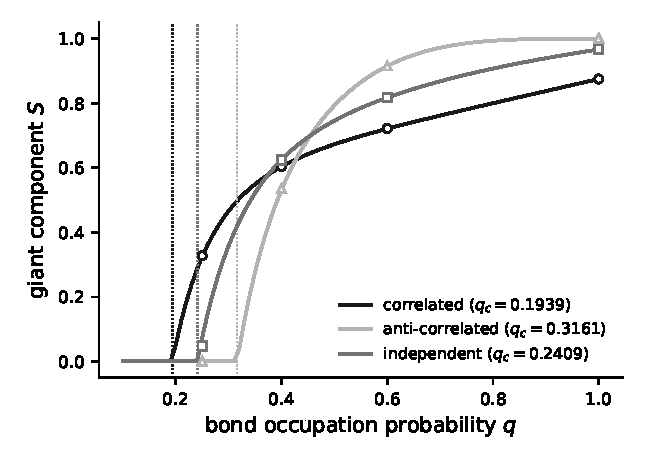
\includegraphics[width=0.9\linewidth]{figs/fig-correlated.pdf}
\caption{\textbf{Identical marginals, three transitions.} Bond percolation on a
graph with links and triangles, for three joint distributions of a node's link
and triangle counts sharing all marginals and therefore every entry of the
published threshold tensor. Lines are Eq.~\eqref{eq:jointmap}, symbols Monte
Carlo at $n=1.5\times10^{5}$, dotted lines the thresholds of
Eq.~\eqref{eq:qc3}. The curves cross between $q=0.38$ and $q=0.46$, so no single statement about
whether correlation helps survives. Generated by
\code{figs/\allowbreak beyond\_\allowbreak threshold.\allowbreak py}.}
\label{fig:correlated}
\end{figure}

The mechanism is intuitive once seen. Positive correlation piles both kinds of
connectivity onto the same nodes, which lowers the threshold --- those nodes
form a well-connected core --- but caps the reachable fraction, because the
complementary nodes are poorly connected in both layers at once.
Anti-correlation spreads connectivity out, raising the threshold but eventually
pulling everything in, $S\to1$ at $q=1$. Neither effect is visible in the first
moments.

\paragraph{One thing to check for.} The fixed point returns the fraction of
complexes in an \emph{infinite} component, which percolation theory identifies
with \emph{the} giant component on the assumption that the infinite component is
unique. Correlated layers can break that. If
$\Phi^{0}(x)=\tfrac12x_{|}^{2}+\tfrac12x_{\triangle}^{2}$ then no node
participates in both layers, the chygraph falls into two disjoint pieces, and
the map returns the sum of their infinite components rather than the larger: at
$q=1$ it reports $S=1$ where simulation gives $1/2$. The decomposition is easy
to test for, and it does not arise when some layer is supercritical on its own
and touches every complex.

\section{Constructions solved by substitution}
\label{sec:constructions}

The point of doing the work once is to be able to stop doing it. Each of the
following has been treated in the literature with a purpose-built calculation,
and each is handled here by writing down the chygraph and substituting.

\subsection{AND-logic against OR-logic}

\citet{bianconi2024} distinguish two rules for what a
higher-order interaction does when some of its members are removed. Under
\emph{OR}-logic the interaction keeps connecting whichever members survive.
Under \emph{AND}-logic it fails outright if any member is missing --- the right
rule for a chemical reaction, a catalytic step, a supply chain.
\citet{ha2025} reach the same distinction independently.

Both are the same chygraph: atoms in layer $0$, hyperedges in layer $1$. They
differ in one generating function,
\begin{equation}
  \bar G^{1}_{0}(y)=
  \begin{cases}
    \bar G_{c}(1-p+py), & \text{OR},\\[2pt]
    1-\bar G_{c}(p)+\bar G_{c}(py), & \text{AND}.
  \end{cases}
  \label{eq:andor}
\end{equation}
Neither $\Phi^{0}_{1}$ nor $\bar\Phi^{0}_{1}$ is thinned, because under either
rule a node reached along a functioning hyperedge is present by construction ---
this is the exception flagged in Sec.~\ref{sec:map}, and node occupation
reappears at the root alone. Nothing downstream knows which rule was chosen.

Differentiating Eq.~\eqref{eq:andor} at $y=1$ reduces the whole difference to
one substitution:
\begin{equation}
  \ave{\bar s}_{10}=p\,\bar G_{c}'(1)\ \text{ (OR)},
  \qquad
  \ave{\bar s}_{10}=p\,\bar G_{c}'(p)\ \text{ (AND)},
  \label{eq:andors}
\end{equation}
the same expression at $1$ and at $p$. Since $\bar G_{c}'$ is a power series
with non-negative coefficients it is non-decreasing on $[0,1]$, so
$\bar G_{c}'(p)\le\bar G_{c}'(1)$ and
\begin{equation}
  \theta_{\mathrm{AND}}\le\theta_{\mathrm{OR}},
  \qquad
  p_{c}^{\mathrm{AND}}\ge p_{c}^{\mathrm{OR}},
\end{equation}
with equality if and only if $p=1$ or $c\equiv2$ --- for an ordinary graph the
two rules are the same statement. That is a one-line proof of the inequality
reported by \citet{bianconi2024}. For Poisson degrees and cardinalities,
$\theta_{\mathrm{OR}}=p\ave{k}\ave{c}-1$ and
$\theta_{\mathrm{AND}}=p\ave{k}\ave{c}e^{\ave{c}(p-1)}-1$; at $\ave{k}=2$,
$\ave{c}=3$ the thresholds are $1/6$ and $0.5827$, more than a factor of three
apart (Fig.~\ref{fig:andor}).

\begin{figure}[t]
\centering
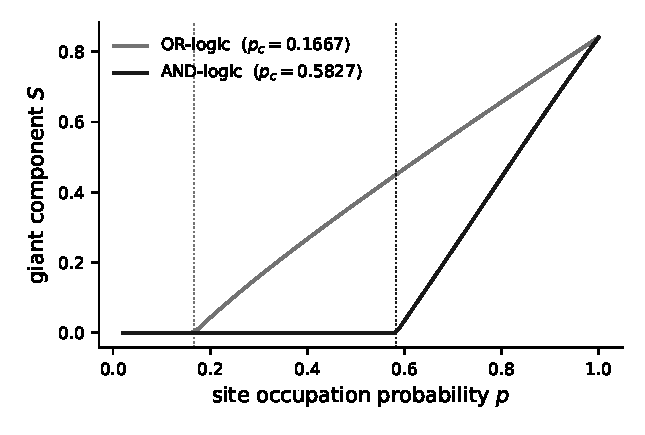
\includegraphics[width=0.9\linewidth]{figs/fig-andor.pdf}
\caption{\textbf{One chygraph, one generating function apart.} Site percolation
on a Poisson hypergraph, $\ave{k}=2$, $\ave{c}=3$, under the two rules of
Eq.~\eqref{eq:andor}: a hyperedge that keeps connecting its survivors, against
one that fails if any member is missing. The thresholds differ by a factor of
$3.5$; the curves must meet at $p=1$, where the rules coincide. Generated by
\code{figs/\allowbreak beyond\_\allowbreak threshold.\allowbreak py}.}
\label{fig:andor}
\end{figure}

\subsection{Hyperdegree--cardinality correlation}

Whether nodes of high hyperdegree join hyperedges of large cardinality is a
measurable property of real hypergraphs and one known to matter
\citep{ha2025,fujiki2018}. It is a correlation between layers in the sense of
Sec.~\ref{sec:joint}: split the hyperedges into layers by cardinality class, and
the joint chy-degree generating function \emph{is} the correlation.

Taking classes $c=2$ and $c=5$ and a one-parameter family in which both marginal
hyperdegree distributions --- and hence the entire published tensor --- are held
fixed while the covariance runs from maximally negative through independent to
maximally positive, the site percolation thresholds are
\begin{equation}
  p_{c}=0.2460,\qquad 0.2120,\qquad 0.1793.
\end{equation}
Positive correlation concentrates connectivity and lowers the threshold, as
before. But the order parameter is not ordered the same way at every $p$: the
three curves cross, and at $p=1/2$ it is the \emph{independent} member that has
the largest giant component, $0.2423$ against $0.2204$ and $0.2369$, while at
$p=1$ the ordering is monotone in the correlation. No single statement that
correlation helps or hurts survives --- which is an argument for computing the
threshold and the order parameter rather than one of them.

\subsection{Clustered graphs, and applying the theory to the right object}

The constructions so far all put the loops \emph{inside} complexes, which is
where the formalism can absorb them. A recent result shows sharply what happens
when they are not.

\citet{cirigliano2025} solves site percolation on Static Triadic
Closure graphs --- built by closing every triad of a treelike backbone $G_{0}$
to form a clustered graph $G_{1}$ --- and finds that heterogeneous mean field,
which is the treelike rewiring preserving only $G_{1}$'s degree distribution,
gets both the threshold and the critical exponents wrong. This is
Sec.~\ref{sec:treebreaks}'s complaint, sharpened.

The obvious chygraph for $G_{1}$ fails too, and it is instructive that it does.
Closing all triads makes every closed neighbourhood a clique, so $G_{1}$ looks
like a hypergraph with nodes as atoms and neighbourhoods as complexes. But every
backbone edge $u\sim v$ then creates a four-cycle $u-C(v)-v-C(u)-u$ in the
incidence structure, and a chygraph is exact only when \emph{that} is locally
treelike --- Sec.~\ref{sec:treelike} again, one level up. For a Poisson backbone
with $\ave{k}=3$ this mapping gives $p_{c}=0.0711$ against the exact $0.0893$,
no improvement on heterogeneous mean field's $0.0635$. The last two are
\citeauthor{cirigliano2025}'s; the exact value is recovered below,
Eq.~\eqref{eq:stcthresh}, by a mapping that does work.

The formalism does cover the problem, but on the \emph{backbone} rather than on
$G_{1}$. Site percolation on $G_{1}$ is equivalent to extended-range percolation
with $R=2$ on $G_{0}$: two occupied nodes are connected when at most one
unoccupied node lies between them. Promote the occupation state to a layer and
one has a three-layer chygraph --- occupied nodes, unoccupied nodes, backbone
edges --- with
\begin{equation}
  \bar G^{2,(0)}(y)=p\,y_{0}+(1-p)\,y_{1},
  \qquad
  \bar G^{2,(1)}(y)=p\,y_{0}+(1-p).
  \label{eq:stc}
\end{equation}
The entire range-$2$ rule is the difference between those two lines: entering an
edge from an unoccupied node, a second unoccupied node in a row kills the path.
That the intra-complex function may depend on the layer one entered from is
precisely the freedom Sec.~\ref{sec:joint} introduced.

The tensor then returns
\begin{equation}
  \begin{aligned}
    \theta&=-b^{2}p^{2}+b(1+b)p-1,\\
    p_{c}&=\frac{(1+b)-\sqrt{(1+b)^{2}-4}}{2b},
  \end{aligned}
  \label{eq:stcthresh}
\end{equation}
with $b=\ave{k(k-1)}/\ave{k}$, which is \citeauthor{cirigliano2025}'s exact result, and an order
parameter agreeing with it to machine precision at every $p$. The exponents
follow from Sec.~\ref{sec:breakdown}: $C$ is finite when the \emph{backbone}
third moment converges, giving $\beta=1$, and diverges otherwise, giving
$\beta=1/(\gamma_{d}-3)$ --- which in terms of the STC degree exponent is
exactly the published table of exact exponents.

That is the point this book keeps arriving at from different directions, and
it is not that mean field always holds. It is that the tree-based calculation
was being applied to the wrong object. Mapping to a chygraph moves the boundary
of what counts as local from ``no loops'' to ``no loops between complexes'', and
the work is finding a representation that respects the second condition. Here
that required leaving $G_{1}$ altogether. Chapter~\ref{ch:overlap} is what
happens when no such representation is available.

\section{Checks}


\checkhead{Known results}
Equation~\eqref{eq:AisJ} is verified entry by entry, symbolically, for every
mapping in Chapter~\ref{ch:percolation}, by comparing the Jacobian of the map
against an independent implementation of the published tensor; the Perron root
reproduces the published pseudo-order parameter through
$\lambda^{2}=\theta+1$. Equation~\eqref{eq:stcthresh} returns
\citeauthor{cirigliano2025}'s exact threshold for static triadic closure, with
an order parameter agreeing with it to machine precision at every $p$, and
Eq.~\eqref{eq:andors} reproduces the inequality of \citet{bianconi2024}.

\checkhead{New results}
The critical amplitude and the dependent-layer construction have no published
counterpart. The closed-form amplitudes are checked against the numerically
solved map, and against an independent evaluation by numerical eigenvectors on
the full unreduced index set, which also confirms that the core reduction is
exact. The joint construction is checked in both directions: with factorised
inputs it reproduces the factorised map to machine precision, and with
correlated inputs against configuration-model simulation over all three
distributions and the whole range of $q$, agreeing within one standard deviation
in every case --- while the marginals-only prediction is outside it in six of
nine. Every number quoted in this chapter is returned by the software, and the
figures are generated by running it.

\checkhead{Partial results}
The closed forms of Table~\ref{tab:amplitudes} hold only where the second
factorial moments converge, and must not be quoted outside that range;
Sec.~\ref{sec:breakdown} says where the expansion announces its own breakdown
and what replaces $\beta=1$ there. The fixed point returns the fraction of
complexes in an infinite component, which is the giant component only if that
component is unique, and Sec.~\ref{sec:joint} exhibits correlated layers where
it is not --- the map reports $S=1$ at $q=1$ where simulation gives $1/2$.
Interdependent networks are outside the class altogether: $\Lambda=0$ does not
locate their transition, and mapping them to chygraphs is not done.
